
\documentclass[11pt]{article}
\usepackage{graphicx}

\title{ROS 2 TUTORIAL}
%\author{christopher.j.erndteman@usace.army.mil}
\author{Christopher Erndteman}
\date{September 2023}

\usepackage[hidelinks]{hyperref}



\usepackage{xcolor}
\usepackage{float}
\usepackage{titlesec}



\newcommand{\cmd}{\textbf{\$: }}
\usepackage{listings}
\usepackage{color}

\definecolor{dkgreen}{rgb}{0,0.6,0}
\definecolor{gray}{rgb}{0.5,0.5,0.5}
\definecolor{mauve}{rgb}{0.58,0,0.82}

\lstset{frame=tb,
  language=bash,
  aboveskip=3mm,
  belowskip=3mm,
  showstringspaces=false,
  columns=flexible,
  basicstyle={\small\ttfamily},
  numbers=none,
  numberstyle=\tiny\color{gray},
  keywordstyle=\color{blue},
  commentstyle=\color{dkgreen},
  stringstyle=\color{mauve},
  breaklines=true,
  breakatwhitespace=true,
  tabsize=3
}



\newcommand{\link}[2]{\textbf{Link: }\textcolor{blue}{\href{#2}{#1}}\footnote{#2}}

\begin{document}
\maketitle
\tableofcontents
\newpage
 
\section{Description}
Welcome to an introductory tutorial to Robot Operating System 2 (ROS 2).
ROS 2 is an open-source set of tools and packages providing roboticists a powerful framework for development and design. This tutorial will focus on the ROS 2 distribution "Humble Hawksbill", commonly referred to as "Humble". Humble is currently compatible with Ubuntu 22.04 and has a projected end of life in May 2027.
The team at Open Robotics have made a comprehensive tutorial on ROS 2.\footnote{https://docs.ros.org/en/humble/index.html} This tutorial stands to build upon the Open Robotics documentation, not replace it entirely. In final, let this stand as a reference sheet to the use of ROS 2.



\section{Installation}
Below is a simplification of the ROS 2 install process for Ubuntu 22.04.
A bash script can be found in addition to these install commands. These commands will not contain debugging information as that can be found on the official ROS 2 Humble documentation: 
\link{ROS 2 Humble Install Documentation}{https://docs.ros.org/en/humble/Installation/Ubuntu-Install-Debians.html}

\pagebreak
\noindent
\subsection{Install Commands: }
\lstset{language=bash}
\begin{lstlisting}
sudo apt install
locale
sudo apt update
sudo apt install locales
sudo locale-gen en_US en_US.UTF-8
sudo update-locale LC_ALL=en_US.UTF-8 LANG=en_US.UTF-8
export LANG=en_US.UTF-8
locale
sudo apt install software-properties-common
sudo add-apt-repository universe
sudo apt update
sudo apt install curl -y 
sudo curl -sSL https://raw.githubusercontent.com/ros/rosdistro/master/ros.key -o /usr/share/keyrings/ros-archive-keyring.gpg
echo "deb [arch=$(dpkg --print-architecture) signed-by=/usr/share/keyrings/ros-archive-keyring.gpg] http://packages.ros.org/ros2/ubuntu $(. /etc/os-release 
echo $UBUNTU_CODENAME) main" | sudo tee /etc/apt/sources.list.d/ros2.list > /dev/null
sudo apt update
sudo apt upgrade
sudo apt install ros-humble-desktop
sudo apt install ros-humble-ros-base
sudo apt install ros-dev-tools
\end{lstlisting}

\subsection{Uninstall Commands: }
\begin{lstlisting}
sudo apt remove ~nros-humble-*
sudo apt autoremove
\end{lstlisting}
\subsection{Workspace Setup}
Similar to ROS 1, ROS 2 depends on being built in a defined directory called a workspace. Creating a workspace is very simple, follow the instructions below to do so.\\
\begin{lstlisting}
mkdir -p ~/ros2_ws/src
cd ~/ros2_ws 
colcon build
\end{lstlisting}

\subsubsection{Source Command: }
The source command is critical for operation of ROS 2 and should be memorized. The source command adds environment variables to your path that allows ROS to function. 

\begin{lstlisting}
source /opt/ros/${Distribution}/setup.bash
\end{lstlisting}
\noindent
In this guide, we are using the ROS 2 Distribution Humble Hawksbill. Thus we simply replace \$\{Distribution\} with humble.\textit{NOTE: This command must be used every time a new terminal window is opened.} This command can be added to your baschrc file to source upon terminal open.\\
\begin{lstlisting}
# Add source command to bashrc file
echo "source /opt/ros/humble/setup.bash" >> ~/.bashrc
\end{lstlisting}




\section{Command Line Tools}
Use of the command line is critical to developing robotics applications with ROS 2. This section will provide a helpful guide to command line tools in ROS 2.
\subsection{Format}
If you are familiar with ROS 1, ROS 2 retains many of the same commands however has a different format. The command format is as follows. \\
\begin{lstlisting}
ros 2 <primary_command> <secondary_command_or_options>
\end{lstlisting}
Example; Launching a ROS 2 package:\\
\begin{lstlisting}
ros 2 launch <package-name> <package-launch-file>
\end{lstlisting}
\subsection{Common ROS 2 Commands}
\begin{table}[H]
	\caption{ROS 2 Humble CL Commands (Frequently Used)}
	\begin{center}
		\begin{tabular}{c|c}
			Primary Command & Secondary Commands List\\
			\hline
			pkg & create, list, executables, prefix, xml\\
			node & info, list\\
			topic & info, list, type, pub, find, echo, hz\\
			service	& call, list, type, find\\
			action & info, list, send\_goal\\
			bag & info, list, play, record, convert, reindex\\
		\end{tabular}
	\end{center}
\textbf{Hint: -h after Primary Command shows list of Secondary Commands with descriptions, -h after Secondary Command shows description and all options.}
\end{table}

\subsection{ROS 2 Doctor}
This command checks over all of the ROS 2 setup details, and provides helpful warnings/errors.
\begin{lstlisting}
# terminal must be sourced first.
ros2 doctor
\end{lstlisting}
If the command above did not work. Try:
\begin{lstlisting}
# terminal must be sourced first.
sudo apt install ros-humble-ros2cli
ros2 doctor
\end{lstlisting}
\link{ROS 2 Doctor Documentation}{https://docs.ros.org/en/humble/Tutorials/Beginner-Client-Libraries/Getting-Started-With-Ros2doctor.html}


\section{ROS 2 Overview}
ROS 2 maintains many of the same implementation ideologies as it's predecessor ROS, while providing additional features and improving previous components. 
\subsection{Nodes}
Modularity is important. Each node should be used for a specific process or job. Nodes can communicate between each other using the publisher/subscriber method, services, or actions. In ROS 2 there is no need for \textit{roscore}. Nodes can be ran by simply calling:
\begin{lstlisting}
ros2 run <node_name>
\end{lstlisting}

Follow the instructions bellow to create a Node in C++.
\lstset{language=bash}
\begin{lstlisting}
cd <workspace>
ros2 pkg create --node-name <name> --licenses <license> --build-type ament_cmake <pkg_name>
\end{lstlisting}

\lstset{language=C++}
\begin{lstlisting}
//creating a node in ROS 2 C++
#include "rclcpp/rclcpp.hpp"

class My_Node : public rclcpp::Node {
	//Implementation of Node goes here.
}
\end{lstlisting}
Follow the instructions bellow to create a Node in Python.
\lstset{language=bash}
\begin{lstlisting}
cd <workspace>
ros2 pkg create --node-name <name> --licenses <license> --build-type ament_python <pkg_name>
\end{lstlisting}
\lstset{language=Python}
\begin{lstlisting}
//creating a node in ROS 2 Python
import rclpy
from rclpy.node import Node

class My_Node (Node):
	//Implementation of Node goes here.
\end{lstlisting}



\begin{figure}[hbtp]
\centering
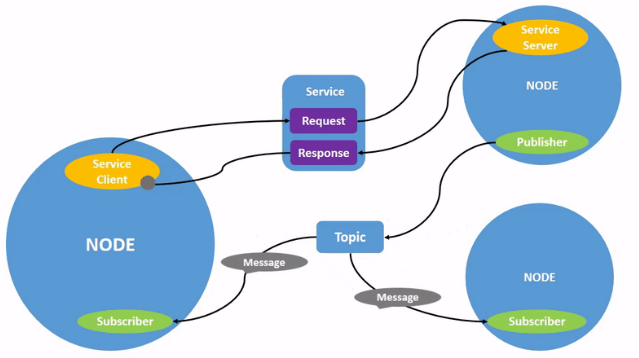
\includegraphics[scale=0.5]{Nodes.png}
\caption{ROS 2 Node layout\\ https://docs.ros.org/en/humble/Tutorials/Beginner-CLI-Tools/Understanding-ROS2-Nodes/Understanding-ROS2-Nodes.html}
\end{figure}
\newpage

\subsection{Publishers \& Subscribers}
Publishers and Subscribers stand as the method of continuous communication between nodes. A foundational idea of publishers and subscribers is that they are not exclusive. Multiple subscribers can subscribe to the same publisher. Additionally, while a subscriber can only subscribe to one publisher, a node can have multiple subscribers.

\subsubsection{Topics}
Topics act as a bus for publisher and subscriber nodes to communicate through. Topics are unique, defined in the publisher node. In order to receive the data the publisher is publishing, the subscriber must subscribe to the defined topic.

\subsubsection{Messages}
Messages contain the data that is being sent via the publisher. Messages are defined types. Messages are custom defined, however many of the needed messages can be found through ROS 2 packages. EX. The std\_msgs package defines messages for many primitive types (ints, bools, strings, etc). There are many more message types for download. Ex. The geometry\_msgs package provides useful messages such as position, Quaternion, etc. For most use cases, a message type is likely to exist. However, if needed, a custom message type can be defined.\\
\link{std\_msgs}{https://index.ros.org/p/std\_msgs/}\\
\link{geometry\_msgs}{https://docs.ros2.org/latest/api/geometry\_msgs/index-msg.html}\\
\link{Custom msgs and srvs in ROS 2 Humble.}{https://docs.ros.org/en/humble/Tutorials/Beginner-Client-Libraries/Custom-ROS2-Interfaces.html}


\subsubsection{Recap}
A publisher will fill a message with data, then the publisher will define the topic that the message will be sent to. Next, the publisher will publish the message on the defined topic. Now, any nodes may define a subscriber which will subscribe to the topic of the defined message type. The ROS 2 Humble documentation offers a full tutorial here: \\
\link{C++ Publisher and Subscriber}{https://docs.ros.org/en/humble/Tutorials/Beginner-Client-Libraries/Writing-A-Simple-Py-Publisher-And-Subscriber.html}\\
\link{Python Publisher and Subscriber}{https://docs.ros.org/en/humble/Tutorials/Beginner-Client-Libraries/Writing-A-Simple-Py-Publisher-And-Subscriber.html}

\subsection{Services and Clients}
Messages may be best requested and responded to, rather than the continuous flow of publishers and subscribers. The service-client model achieves this well. A node defines a service, this service can then be called by any other nodes. A client is created within a node that allows it to call a given service. The most common use of a service is as follows: Client sends a request (often containing data to be processed), service sends a response (the return value of the data that was processed). A request and/or response can be empty, often used for triggering something. \\

\begin{figure}[hbtp]
\centering
\includegraphics[scale=0.4]{../../Pictures/Screenshots/service_client.png}
\caption{ROS 2 Service-Client Example\\ https://docs.ros.org/en/humble/Tutorials/Beginner-CLI-Tools/Understanding-ROS2-Services/Understanding-ROS2-Services.html}
\end{figure}
\pagebreak


%STILL NEED ACTIONS

\subsection{Additional Features}
These features have many use cases. However they do not warrant, or are too expansive for, explanation beyond that of the ROS 2 Humble documentation. Once you are comfortable with the other content covered in the tutorial, come back and explore these features!
\subsubsection{Parameters}
Parameters are variables within the code that can be set in the launch file of a node, allowing for easy tuning.\\
\link{Parameters in Python}{https://docs.ros.org/en/humble/Tutorials/Beginner-Client-Libraries/Using-Parameters-In-A-Class-Python.html}\\
\link{Parameters in C++}{https://docs.ros.org/en/humble/Tutorials/Beginner-Client-Libraries/Using-Parameters-In-A-Class-CPP.html}\\
\subsubsection{tf2}
tf2 let's robotics developers manage multiple coordinate frames. tf2 is an expansive topic and a small explanation would not do it justice. Thus, the best way to learn about tf2 is through the official documentation.\\
\link{tf2 official documentation}{https://docs.ros.org/en/humble/Tutorials/Intermediate/Tf2/Tf2-Main.html\#}\\
\subsubsection{URDF (Unified Robotics Description Format)}
UDRF's are crucial for robotic simulation, however that is beyond the scope of this tutorial.\\
\link{URDF Tutorial}{https://docs.ros.org/en/humble/Tutorials/Intermediate/URDF/URDF-Main.html}\\
\subsubsection{Quality of Service settings}
Quality of Service in ROS 2 allows the developer to tune communication between nodes. ROS 2 offers a plethora of QoS settings, including "Best effort", "Reliable", and many more.\\
\link{QoS official documentation}{https://docs.ros.org/en/humble/Concepts/Intermediate/About-Quality-of-Service-Settings.html\#qos-policies}\\

\subsection{Actions}
Actions are back and better than ever! Action servers existed in ROS 1 through the actionlib library, however are now a full feature of ROS 2. Actions are very similar to services/clients, however provide feedback while running. Similar to ROS 1, actions are often used for wave-point navigation or other processes that take a large amount of time. Actions allow the client of the action to cancel the action mid process. 

\subsubsection{Defining an action}
\lstset{language=c++}
\begin{lstlisting}
# Request
---
# Result
---
# Feedback
\end{lstlisting}
Ex. Navigating to wave-point:
\begin{lstlisting}
float64[] goal_coordinates
---
bool success
---
float64[] current_coordinates
\end{lstlisting} 
As you can see above this is very similar to the custom msgs and custom srvs implementation.\\
\link{Read here for building actions}{https://docs.ros.org/en/humble/Tutorials/Intermediate/Creating-an-Action.html}\\
\link{Basic data types for actions, msgs, and srvs}{https://docs.ros.org/en/humble/Concepts/Basic/About-Interfaces.html}\\

\subsubsection{Creating Action Servers and Clients}


\subsection{Launch Files}
Launch files can be used to run multiple nodes with one command. A crucial part of any ROS 2 stack, launch files allow for parameter adjustment as well as running nodes. ROS 2 launch files can be created using Python, XML, or YAML. In this tutorial we will focus on Python launch files.\\
\subsubsection{Creating Launch Files}
Launch files should go in a directory named launch in your ROS 2 workspace. 
\lstset{language=bash}
\begin{lstlisting}
cd ~/ros2_ws
mkdir launch
touch my_launch_file.launch.py
\end{lstlisting}
\pagebreak

\subsubsection{Writing Python Launch File}
\lstset{language=python}
\begin{lstlisting}
from launch import LaunchDescription
from launch_ros.actions import Node

def generate_launch_description():
    return LaunchDescription([    
    
    # Define the value of a parameter in the launch file.
    DeclareLaunchArgument('example_parameter', default_value='20') 
    
############ Example of launching two of the same node ##########        
        Node(
            package='example_package_name_1',
            namespace='namespace_1',
            executable='ex_pkg_node',
            name='example'
        ),
        Node(
            package='example_package_name_1',
            namespace='namespace_1_2',
            executable='ex_pkg_node',
            name='example'
        )
#################################################################

########### Example launching different nodes ###################
		Node(
            package='example_package_name_2',
            namespace='namespace_2',
            executable='ex_pkg_node_2',
            name='example_2'
        ),
        Node(
            package='example_package_name_3',
            namespace='namespace_3',
            executable='ex_pkg_node_3',
            name='example_3',
            # Use the example_parameter from our configuration above.
            parameters=[{'example_parameter': LaunchConfiguration('example_parameter')}] 
        )
#################################################################
    ])
\end{lstlisting}
Explanation:\\
\textbf{package} - This is the name of the package you want to launch.\\
\textbf{namespace} - Namespaces allow you to create multiple instances of the same node.\\
\textbf{executable }- This can be found in the setup.py file for your package inside entry\_points=\{\}, for C++ this can be found in the add\_executable() command in CMakeLists.txt.\\
\textbf{name} - This is simply what the instance of that node will be called, it must be unique.\\
\textbf{parameters} - Use parameters to tune your code, these must be defined within your node. Change the values within the launch file shown above to change the value in the code.\\

\section{Tutorial Project}
The ROS 2 Humble official documentation has a tutorial for you to complete.\footnote{https://docs.ros.org/en/humble/Tutorials/Beginner-Client-Libraries.html} This tutorial is designed to supplement the ROS 2 official tutorial and provide an opportunity to create code using the ROS 2 framework. Robotics knowledge is not required nor utilized in this project. The project goal is to have you use as many aspects of the ROS 2 framework as possible.

\subsection{Project Overview}
You're the owner, and only employee, of a pizza-tech restaurant startup! However, your restaurant only does delivery. You're in luck, in the modern world everyone uses robots for their daily life, and all of the robots run on ROS 2 Humble. Your goal, make the most money!

\subsection{Getting Started}
\lstset{language=bash}
\begin{lstlisting}
cd ~	
\end{lstlisting}
Start by going into the home directory.\\
\begin{lstlisting}
mkdir ros2_tutorial_ws 
cd ~/ros2_tutorial_ws	
\end{lstlisting}
Create your ROS 2 workspace directory for the tutorial project, then change into the workspace directory.\\

\begin{lstlisting}
git clone <github tutorial files location> . 
\end{lstlisting}
The tutorial contains both a src directory and a launch directory. These directories contain everything needed to build and start the simulation. Clone from the github remote where the files are located, make sure to use the . after your clone to clone the files directly into your ros2\_tutorial\_ws directory.\\

\begin{lstlisting}
colcon build
source /opt/ros/humble/setup.bash
source install/setup.bash
\end{lstlisting}
Build and source, this should all be done in ~/ros2\_tutorial\_ws\\
\begin{lstlisting}
cd launch
ros2 launch pizza_sim.launch.py
\end{lstlisting}
Change into the launch directory and launch the pizza simulation.\\
\begin{lstlisting}
cd ~/ros2_tutorial_ws
source /opt/ros/humble/setup.bash
\end{lstlisting}
Open a new terminal, source it and begin working through the tutorial.\\
\begin{lstlisting}
cd ~/ros2_tutorial_ws/src
ros2 pkg create --build-type ament_cmake --dependencies rclcpp rclpy std_msgs msgs_and_srvs rclcpp_action --license Apache-2.0 delivery_client
\end{lstlisting}
Create your ROS 2 package inside your src directory, you can change the --build-type argument to ament\_python for python use. \\

\noindent \textit{Hint:}\\
Use the command-line to gain as much information about the pizza business before you create your own node. As a hint, start with this command:\\
\begin{lstlisting}
ros2 node list
# For more call:
ros2 --help
\end{lstlisting}

\subsection{Ingredients: Publishers and Subscribers}
Before you can serve to customers, you need to receive ingredients from your suppliers. Both of your suppliers use ROS 2 to deliever their digital ingredients. The /crust\_supplier, and /toppings\_supplier nodes are publishers of their ingredients. Use the command-line to find what topics they publish to. Use the tutorials below to guide you in subscribing to these topics. Create one node that subscribes to both topics. Note, the crust and toppings suppliers aren't consistent. You'll need to save the data you receive for later use, and/or check that the supplies match the customers order.\\
\link{C++ Publisher and Subscriber}{https://docs.ros.org/en/humble/Tutorials/Beginner-Client-Libraries/Writing-A-Simple-Py-Publisher-And-Subscriber.html}\\
\link{Python Publisher and Subscriber}{https://docs.ros.org/en/humble/Tutorials/Beginner-Client-Libraries/Writing-A-Simple-Py-Publisher-And-Subscriber.html}\\
\textbf{Important: This tutorial uses custom msg types. These msg files can be found in src/msgs\_and\_srvs/msg of the ros2\_tutorial\_ws.}\\
The crust supplier publishes a Crust msg. The toppings supplier publishes a Toppings msg. Look in these msg files to see what they contain.\\
\link{Custom msgs and srvs in ROS 2 Humble.}{https://docs.ros.org/en/humble/Tutorials/Beginner-Client-Libraries/Custom-ROS2-Interfaces.html}

\lstset{language=python}
\begin{lstlisting}
# How to include msg and srvs files in python
from msgs_and_srvs.msg import Crust, Toppings
from msgs_and_srvs.srv import Order
\end{lstlisting}

\lstset{language=c++}
\begin{lstlisting}
// How to include msg and srvs files in c++
#include "msgs_and_srvs/msg/Crust.hpp"
#include "msgs_and_srvs/msg/Toppings.hpp"
#include "msgs_and_srvs/srv/Order.hpp"
\end{lstlisting}

\subsection{Customer Order: Services and Clients}
Now you have ingredients, all that's left is to make the pizza and send it to customers. However, you must know what pizza the customer wants before you make it. Create a service (within the same node) that takes in a order and payment, then returns the pizza. Use the Order.srv file in the msgs\_and\_srvs directory. \textbf{The topic of the service must be "order". If this is not the case the tutorial client will not be able to find your restaurant.}\\
\noindent
\link{C++ Service and Client}{https://docs.ros.org/en/humble/Tutorials/Beginner-Client-Libraries/Writing-A-Simple-Cpp-Service-And-Client.html}\\
\link{Python Service and Client}{https://docs.ros.org/en/humble/Tutorials/Beginner-Client-Libraries/Writing-A-Simple-Py-Service-And-Client.html}

\subsubsection{Building a pizza}
As you may see in the Order.srv and Payment.srv files, there is a field called pizza\_id. This lets the tutorial verify the correct means were used to build the pizza (Anti-cheat method). To get the pizza\_id, multiply the toppings\_id, and crust\_id.


\subsection{Using Actions: Delivery Man}
Your pizza shop is thriving, now it's time to use an additional feature of ROS 2 to make extra money. Create a ROS 2 action client within your node, that calls the delivery\_man action server. Send the delivery man a pizza, then watch the feedback for the customers patience level. If the patience level has gone to 0 this means the customer will not take the pizza, you must cancel the order and send a new request to the delivery\_man action server. You can find the action file in msgs\_and\_srvs/action/Delivery.action. When the action server returns, add the payment to your total.\\


\end{document}
